No, it is not since $(A,F,C,G)$ is a 4-cycle that is not triangulated. Added edges are in green to moralize the graph.

\begin{center}
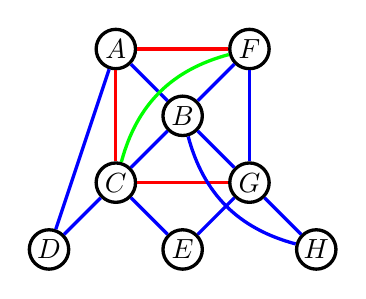
\begin{tikzpicture}[>=stealth, node distance=1.2cm]
    \tikzstyle{format} = [draw, very thick, circle, minimum size=5.0mm,
	inner sep=0pt]

	\begin{scope}
		\path[-, very thick]
			node[format] (A) {$A$}
			node[format, below right of=A] (B) {$B$}
			node[format, below left of=B] (C) {$C$}
			node[format, below left of=C] (D) {$D$}
			node[format, below right of=C] (E) {$E$}
			
			node[format, above right of=B] (F) {$F$}
			node[format, below right of=B] (G) {$G$}
			node[format, below right of=G] (H) {$H$}

			(A) edge[blue] (B)
			(B) edge[blue] (C)
			(A) edge[red]  (C)
			(A) edge[red]  (F)
			

			(C) edge[blue] (D)
			(C) edge[blue] (E)
			(C) edge[red]  (G)

			(F) edge[blue] (B)
			(B) edge[blue] (G)
			(G) edge[blue] (H)
			
			(A) edge[blue] (D)
			(B) edge[blue, bend right=30] (H)
			(F) edge[blue] (G)
			(G) edge[blue] (E)
			
			(F) edge[green, bend right=30] (C)
		;
	\end{scope}
\end{tikzpicture}
\end{center}

Maximal Cliques: 
$(A,B,C,F), (B,C,F,G), (A,C,D), (C,E,G), (B,G,H)$

The new factorization is:
\begin{equation*}
    p(A,B,C,D,E,F,G,H) = \frac{1}{Z} \clique{ABCF}\clique{BCFG}\clique{ACD}\clique{CEG}\clique{BGH}
\end{equation*}
